% !TEX root = QlockToo.tex
% Kapitelvorlage

\section{Einleitung}
\label{sec:Einleitung}
\begin{figure}[h!]
    \centering
    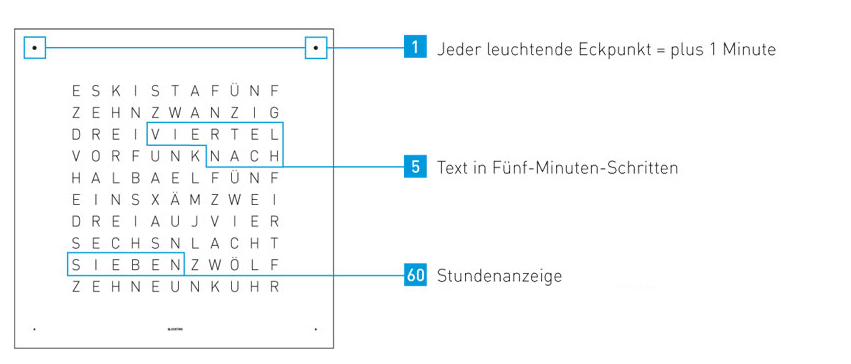
\includegraphics[width=\textwidth]{Abbildungen/Uhrzeit_Beispiel}
    \caption[Uhrzeit_Bspl]{Beispiel: 7 Uhr 17}
    \label{fig:Uhrzeit_Bspl}
\end{figure}
%
In der heutigen Zeit steht neben der Funktionalität vieler Dinge ihr Design im Vordergrund. Bestes Beispiel ist die CLOCKTWO® der Biegert \&  Funk Manufacture GmbH \& Co. KG. Mit dem Slogan  \textit{Zeit in zeitlosem Design}  bewirbt die Designmanufaktur die außergewöhnliche Uhr.
%
\begin{figure}[h]
    \centering
    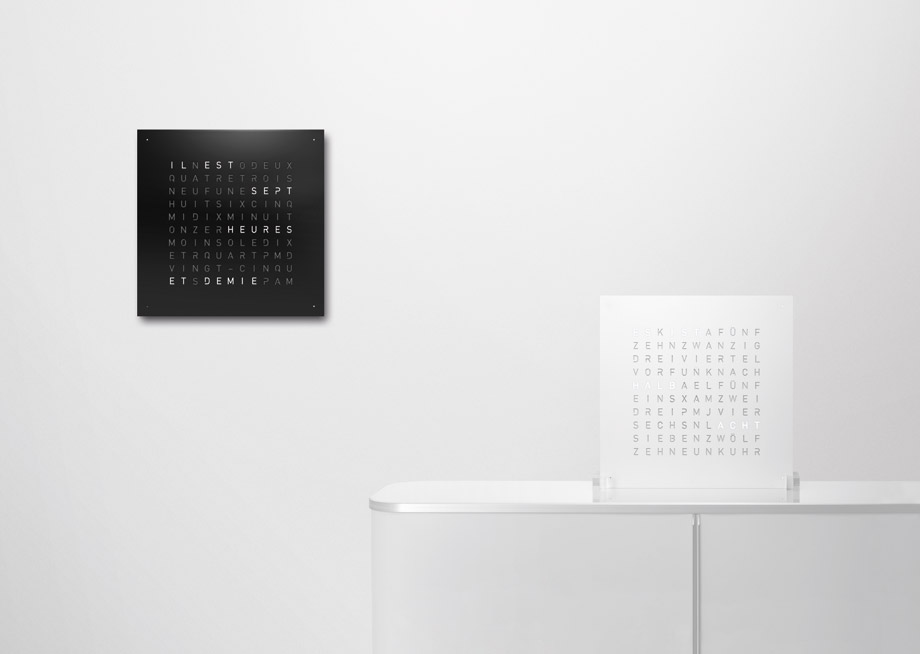
\includegraphics[width=\columnwidth]{Abbildungen/29}
    \caption[ClockTwo]{CLOCKTWO CLASSIC}
    \label{fig:Verbindungsdialog}
\end{figure}

\begin{multicols}{2}
Die QLOCKTWO® ist ein international eingetragenes Markenzeichen, welches zudem durch internationale Patente und Designpatente geschützt ist. Inspiriert durch diese einzigartigen Darstellung der Zeit in geschriebenen Worten, entsteht das Entwicklungs- und Fertigungskonzept einer elektronischen Wanduhr mit einer LED-Matrix. \textit{We can built a CLOCK,TOO.}
%
Die Zeitanzeige erfolgt in Fünf-Minuten-Schritten mit Worten. Diese werden durch das Schalten von LEDs hinter einer Buchstabenmatrix auf einem Frontcover aus Plexiglas ausgeleuchtet. Vier zusätzliche Leuchtpunkte in den Ecken zeigen die Minuten dazwischen.
\end{multicols}





\subsection{Unterkapitel}

